\chapter{Methodology}\label{cap:methodology}

%Nessa dissertação, propõe-se uma metodologia para a análise de risco em projetos de software, a partir de dados históricos de registros de riscos, por meio da utilização de redes neurais artificiais. Para desenvolver essa metodologia, primeiramente necessita-se de uma base de dados extensa e real de riscos em projetos de software. No entanto, há uma dificuldade em encontrar publicamente bases de dados representativas e confiáveis. Uma base de dados de risco chamada PERIL \cite{kendrick2003identifying} mostrou atender as necessidades básicas para essa pesquisa, além de já estar totalmente classificada (mais detalhes na Seção \ref{sec:perildataset}). Nesse estudo, precisa-se de uma base de dados extensa de registros de riscos oriundos de diversos projetos espalhados pelo mundo e em diversos períodos de tempo, com o objetivo de mostrar evidências de quais são os principais modos de falha em projetos e um padrão para explorar respostas aos riscos.
In this dissertation, it is proposed a methodology for risk analysis in software projects, from historical database of risk registers, through the use of artificial neural networks. To develop this methodology, first it is needed an extensive and real database of risks in software projects. However, there is a difficulty in finding publicly bases of representative and reliable data. A database called risk PERIL \cite{kendrick2003identifying} showed  to meet basic needs for this research, in addition to already be fully classified (more details in Section \ref{sec:perildataset}). This study requires an extensive database of risk registers from various projects around the world and in different time periods in order to show evidence of which are the main modes of failure in projects and a standard for explore risk responses.

%Segundo, é necessário realizar o pré-processamento dos dados para que as variáveis de entradas sejam transformadas, normalizadas e selecionadas para o estudo. Terceiro, avaliar o desempenho das ferramentas de estado da arte quanto ao erro de previsão: Simulação de Monte Carlo e Análise PERT.
Second, it is necessary to perform data preprocessing for input variables to be converted into numeric, standardized and selected for the study. Third, evaluate the performance of state of the art tools about forecast error, Monte Carlo simulation and PERT Analysis.

%Quarto, implementar cada modelo de previsão para que pudéssemos selecionar o melhor modelo em redes neurais artificiais: Perceptron de Múltiplas Camadas, Máquinas de Vetor de Suporte, Redes de Função de Base Radial e o Sistema de Inferência Adaptativo Neuro-Fuzzy. Alguns desses modelos selecionados apresentam alguns parâmetros e devido a diversidade de possíveis valores para cada parâmetro, necessita-se otimizar os parâmetros dos modelos. Nesse estudo, implementa-se uma variação da meta-heurística Otimização por Enxame de Partículas (PSO - \textit{Particle Swarm Optimization}) com coeficiente de constrição de Clerk \cite{engelbrecht2007computational} para realizar a tarefa de otimização dos parâmetros das RNAs. O espaço de busca do problema de otimização desses parâmetros é multi-dimensional, complexo e apresenta diversos mínimos locais. 
Fourth, implement each prediction model so we could select the best model in artificial neural networks: Multilayer Perceptron, Support Vector Machine, Radial Basis Function and the Adaptive Neuro-Fuzzy Inference System. Some of these selected models have some parameters and due to the diversity of possible values for each parameter, one needs to optimize the parameters of the models. This study implements a variation of meta-heuristic Particle Swarm Optimization (PSO) with a constriction coefficient of Clerk \cite{engelbrecht2007computational} to accomplish the task of optimizing the parameters of ANNs. The search space of the problem of optimization of these parameters is multi-dimensional, complex and has many local minima.

%Na Figura \ref{fig:method2}, observa-se um esquema ilustrando que um algoritmo de otimização executa os quatro modelos em suas diversas configurações paramétricas para que seja possível eleger o modelo mais eficiente para a base de dados adotada.
In Figure \ref{fig:method2}, it is observed a schematic showing that an optimization algorithm performs the four models in its various parametric settings so you can choose the most efficient model for the chosen database.

\begin{figure}[h]
	\centering
	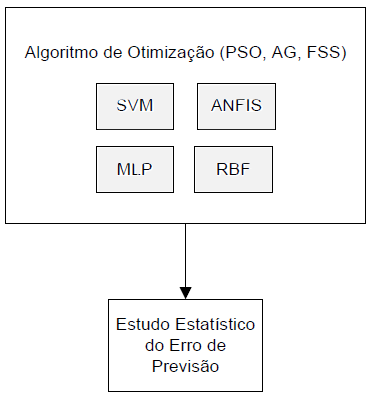
\includegraphics[width=.45\textwidth]{image/MetodologiaDissertacao2.png}
	%\caption{Esquema de Seleção da Melhor Rede Neural Artificial}
	\caption{Schema for selection of best ANN}
	\label{fig:method2}
\end{figure}

%Quinto, um teste de validação dos resultados é realizado para verificar se os modelos baseados em redes neurais artificiais apresentam menor erro que os modelos de estado da arte em análise de riscos: Simulação de Monte Carlo, Análise PERT, Modelo de Regressão Linear Múltipla, Modelo de Regressão em Árvore. Os dois últimos modelos de regressão linear foram considerados como linha de base, por serem modelos mais simples, já que realizam a regressão linear. Os dois últimos modelos foram implementados e também são avaliados quanto ao erro na previsão.
Fifth, a validation test of outcomes is carried out to check whether models based on artificial neural networks have lower error than state of the art models in risk analysis: Monte Carlo Simulation, PERT Analysis, Multiple Linear Regression, Regression Tree Model. The first two models have been implemented and are also evaluated for error in prediction. The last two, were considered baseline for being simpler models since they perform linear regression.

%A seleção do melhor modelo é feita em termos da precisão na estimativa dos impactos dos riscos. É difícil obter uma métrica representativa da precisão de um modelo. No entanto, Engelbrecht \cite{engelbrecht2007computational} e Saxena \cite{saxena2012software} sugerem que a Raiz do Erro Médio Quadrático(REMQ) é uma medida conveniente e aplicável para a maioria dos problemas. A precisão, nesse caso, significa o grau de proximidade de uma saída calculada para a esperada. A REMQ é representada pela Equação \ref{eq:RMSE}:
The selection of the best model is made in terms of accuracy in estimating the impacts of risks. It is difficult to obtain a representative measure of the accuracy of a model. However, Engelbrecht \cite{engelbrecht2007computational} and Saxena \cite{saxena2012software} suggest that the Root Mean Square Error (RMSE) is a convenient measure applicable to most problems. Accuracy in this case means the degree of closeness calculated for an expected output. RMSE is represented by Equation \ref{eq:RMSE}:

\begin{equation}\label{eq:RMSE}
    REMQ= \sqrt[2]{\frac{1}{n}\sum_{i=1}^{n} (e_i)^2},
\end{equation}

%onde $e_i=f_i - y_i$, $f_i$ é o resultado calculado, $y_i$ é o resultado esperado e $n$ é o número de tuplas de dados.
where $e_i=f_i - y_i$, $f_i$ is the calculated outcome, $y_i$ is the expected outcome and $n$ is the number of data pairs.

%Todas as técnicas estudadas nesse trabalho estimam a saída para o impacto de riscos, a REMQ é calculada trinta vezes para cada abordagem e um Teste Estatístico de Wilcoxon Não-pareado \cite{siegel1956nonparametric} pode ser necessário para determinar qual é uma abordagem mais precisa para a base de dados (nesse estudo, o PERIL). O Teste de Wilcoxon não-pareado é utilizado porque não há evidências que as amostras sejam oriundas de uma população normalmente distribuída, como também não há relação de ordem nos valores pertencentes às amostras.
The eight selected techniques have predicted the outcome to risk impacts. Root Mean Square Error is calculated thirty times for each method. Nevertheless, a Non-paired Wilcoxon Test \cite{siegel1956nonparametric} may be necessary to assert which is a more efficient approach to fit dataset (e.g. PERIL). Non-paired Wilcoxon Test is used because there were no evidence that the samples came from a normally distributed population, either there were no relation between outcomes from different samples.

%A validação cruzada \cite{amari1996statistical} é utilizada para evitar a ocorrência de \textit{overfitting} ou \textit{underfitting} durante o treinamento das RNA's. Nesse caso, um treinamento com parada prematura é utilizado para identificar o início do \textit{overfitting}, já que esse método tem provado ser capaz de melhorar a capacidade de generalização da RNA em comparação com o treinamento exaustivo \cite{haykin-1994} \cite{engelbrecht2007computational} \cite{amari1996new}. Portanto, o método de validação cruzada é utilizado para cada abordagem, excluindo a Simulação de Monte Carlo e Análise PERT, para promover maior capacidade de generalização. Quando adotamos o uso da validação cruzada, significa que necessitamos particionar a base de dados em três partes: conjunto de treinamento, conjunto de validação cruzada e conjunto de testes. O conjunto de treinamento é utilizado na fase de treinamento das RNA's, momento em que o aprendizado ocorre. O conjunto de validação cruzada é processado ao mesmo tempo, com o conjunto de treinamento e determina a parada no treinamento. Já o conjunto de testes, é utilizado para produzir a métrica de precisão do modelo, o REMQ.
Furthermore, cross-validation \cite{amari1996statistical} must be used to avoid the occurrence of overfitting or underfitting of data training. In this situation \textit{early stopping} training is used to identify the beginning of overfitting because this method has been proved to be capable of improving the generalization performance of the ANN over exhaustive training \cite{haykin1994neural} \cite{engelbrecht2007computational} \cite{amari1996new}. Therefore, cross-validation method is used for each alternative, excluding Monte Carlo Simulation and PERT Analysis, to promote higher generalization performance. When cross-validation is adopted, it means that it is needed to partition the database into three disjoint groups: training, cross-validation and test subset. Training set is used in training phase the RNA's, at which learning takes place. Cross-validation subset is processed simultaneously with training subset and determine the stop in network training since test subset is used to obtain accuracy of the model, RMSE.

%Por fim, a previsão do impacto do risco e a definição de um intervalo de confiança para uma amostra do conjunto de treinamento são obtidas utilizando o modelo de previsão mais preciso após os testes de validação. É necessário um intervalo de confiança da previsão para que os gerentes de projetos e analistas de risco possam estabelecer o nível de confiança de acordo com a sua necessidade. Afinal de contas, esse é o resultado que eles esperam.
Finally, risk impact estimation and establishment of a confidence interval for a sample of the training set are obtained using the most accurate prediction model after validation tests. It is necessary to define a confidence interval of prediction for project managers and risk analysts establish the confidence level according to their needs. After all, this is the result they expect.

%A Figura \ref{fig:method} apresenta um fluxograma com a metodologia estabelecida para esse estudo. O procedimento inicia-se com a seleção da base de dados que serve como conjunto de dados de entrada, nesse caso o PERIL, e finaliza com a atividade "Definição do Intervalo de Confiança". Todas as atividades são executadas sequencialmente, exceto as atividades "Avaliação dos Modelos de Estado da Arte" e "Seleção da Melhor Rede Neural Artificial" que são executados paralelamente.
Figure \ref{fig:method} presents a flowchart with the established methodology for this study. The procedure begins with the selection of the database that serves as a set of input data, in this case the PERIL, and ends with the activity "Definition of Confidence Interval". All activities are executed sequentially, except activities "Evaluation of Models of State of the Art" and "Best Selection of Artificial Neural Network" that run in parallel. 

\begin{figure}[h]
	\centering
	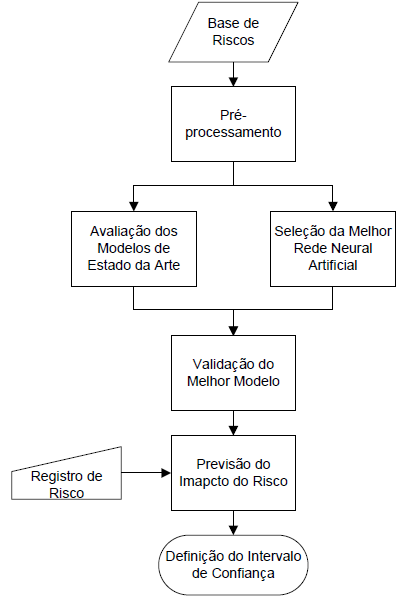
\includegraphics[width=.45\textwidth]{image/MetodologiaDissertacao.png}
%	\caption{Fluxograma do estudo realizado}
	\caption{Flowchart of performed study}
	\label{fig:method}
\end{figure}

\section{PERIL Database}
\label{sec:perildataset}

A better risk management starts identifying potential problems, asserted here as risk factors. The adoption of available methods like: reviewing learned lessons, brainstorming, interviews and specialized judgment are suposed to be relative efficient alternatives, otherwise in most of situations it involves high costs. A low cost, extensive and accessible proposal is to utilize Project Experience Risk Information Library (PERIL) database \cite{kendrick2003identifying}. PERIL database provides information and experience of other project risk management.
%Um melhor gerenciamento de riscos inicia com a identificação de problemas potenciais, atribuído como fatores de risco. A adoção dos métodos disponíveis como: revisar lições aprendidas, \textit{brainstorming}, entrevistas e opinião especializada são alternativas relativamente eficientes, no entanto, na maioria das situações elas envolvem alto custo. Uma proposta de baixo custo, extensiva e acessível é utilizar a base de dados \textit{Project Experience Risk Information Library}(PERIL) \cite{kendrick2003identifying}. A base de dados PERIL provê informações e experiências de outras gestões de risco de projetos.

For more than a decade, in Risk Management Workshops, Kendrick have collected anonymous data from hundred of project leaders dealing with their past project problems. He has compiled this data in the PERIL database, which summarizes both a description of what went wrong and the amount of impact it had on each project. The dataset provides a sobering perspective on what future projects may face and is valuable in helping to identify at least some of what might otherwise be invisible risks or black swans \cite{kendrick2003identifying}.
%Por mais de uma década, durante \textit{Workshops} de Gerenciamento de Riscos, Kendrick coletou dados anônimos de centenas de líderes de projetos lidando com seus problemas em projetos passados. Ele compilou essas informações na base de dados PERIL, que sumariza tanto uma descrição do que houve de errado quanto o impacto que ele teve em cada projeto. A base provê uma perspectiva preocupante do que projetos futuros podem encarar e é valiosa na ajuda para a identificação do que pelo menos poderiam ter sido riscos invisíveis ou \textit{black swans} \cite{kendrick2003identifying}.

According to Kendrick, in projects, the identified risks can be classified as "known", those anticipated during planning, or "unknown" further identified during project execution. The purpose of this dataset is to provide a framework to identify risks, in such a way to increase the number of "known", and decrease the amount of "unknown" risks \cite{kendrick2003identifying}.
%Segundo Kendrick, em projetos, os riscos identificados podem ser classificados como "conhecidos", aqueles antecipados durante o planejamento, ou "desconhecidos", identificados futuramente durante a execução do projeto. O propósito dessa base de dados é prover um \textit{framework} para identificar riscos, de modo a aumentar o número de "conhecidos" e diminuir o número de "desconhecidos" \cite{kendrick2003identifying}.

Some characteristics of PERIL are: 
\begin{itemize}
\item the data are not relational, they contain only a small fraction of the tens of thousands projects undertaken by the project leaders from whom they were collected;
\item they present bias, the information was not collected randomly;
\item they represent only the most significant risks;
\item they are worldwide, with a majority from the Americas;
\item they do not identify opportunities; 
\item they contain six hundred and forty nine registers, whose relative impact is based on the number of weeks delayed the project schedule;
\item typical project had a planned duration between six months and one year;
\item typical staffing was rarely larger than about twenty people.
\end{itemize}
%Algumas características da PERIL são:
%\begin{itemize}
%\item Os dados não estão relacionados, eles representam somente uma pequena fração de dezenas de milhares de projetos realizados pelos líderes de projetos, cujos riscos foram coletados;
%\item Apresentam viés, a informação não foi coletada aleatoriamente;
%\item Representam somente os riscos mais significativos;
%\item São de todo o mundo, com a maioria nas Américas;
%\item Não identificam oportunidades; 
%\item Contém seis centos e quarenta e nove registros, cujo impacto relativo é baseado no número de semanas de atraso no cronograma;
%\item Projetos comuns tiveram um cronograma inicialmente planejado entre seis meses e um ano;
%\item Tamanho da equipe raramente foi maior que vinte pessoas.
%\end{itemize}

Risk registers are categorized as scope, schedule and resource. Scope is decomposed in change and defect subcategories. Schedule is decomposed in dependency, estimative and delay subcategories. Resources is decomposed in money, outsourcing and people subcategories. One benefit of PERIL is that the author contemplates "black swans": risks with large impact, difficult to predict and with rare occurrence \cite{taleb2001fooled}. 
%Os registros de risco são categorizados em escopo, cronograma e recurso. O escopo é decomposto nas subcategorias mudança e defeito. O cronograma é decomposto em dependência, estimativa e atraso. Os recursos são decompostos em dinheiro, \textit{outsourcing} e pessoas. Um benefício da PERIL é que o autor contempla "\textit{black swans}": riscos com grande impacto, difíceis de prever e com ocorrência rara \cite{taleb2001fooled}.

Kendrick chose to normalize all the quantitative data using only time impact, measured in weeks of project slippage. This tactic made sense in light of today's obsession with meeting deadlines, and it was an easy choice because by far the most prevalent serious impact reported in this data was deadline slip. Focusing on time is also appropriate because among the project triple constraints of scope, time ans cost, time is the only one that's completely out of our control - when it's gone, it's gone \cite{KEND2003BOOK}.
%Kendrick decidiu padronizar o impacto usando como métrica o tempo, medido em semanas de atraso no projeto. Essa tática faz sentido à luz da obsessão de hoje por cumprimento de prazos e foi uma escolha fácil, pois, de longe, o impacto mais sério relatado nesses dados foi o atraso no prazo. Focar-se em tempo também é apropriado porque entre as restrições triplas de projeto - escopo, tempo e custo -, tempo é o único é completamente fora de nosso controle. Afinal, quando se vai, se foi \cite{KEND2003BOOK}.

%\begin{table}[h]
%\caption{Impacto total de projetos pelas causas-raiz de categorias e subcategorias %\cite{KEND2003BOOK}}\label{tab:peril_pareto} \centering
%\begin{tabular}{|l|c|c|c|c|}
% \hline
% Subcat. & & & Impacto & Impacto \\
% Causas-raiz & Definição & Casos & Cumul. & Médio \\
% \hline
%  Escopo: & Revisão no escopo &  &  &  \\
%  Mudanças & durante o projeto & 177 & 1460 & 8,2 \\
% \hline
%  Recurso: &  &  &  &  \\
%  Pessoas & Problemas de relacionamento interno & 123 & 706 & 5,7 \\
% \hline
%  Escopo: & Falha em alcançar  &  &  &  \\
%  Defeito & requisitos de entrega & 93 & 654 & 7,0 \\
% \hline
%  Cronograma: & Atraso devido a fatores &  &  &  \\
%  Atrasos & sob o controle do projeto & 102 & 509 & 5,0 \\
% \hline
%  Cronograma: & Durações inadequadas alocadas &  &  &  \\
%  Estimativas & para atividades do projeto & 49 & 370 & 7,6 \\
% \hline
%  Recurso: &  &  &  &  \\
%  \textit{Outsourcing} & Problemas de relacionamento externo & 47 & 316 & 6,7 \\
% \hline
%  Cronograma: & Atraso no projeto devido &  &  &  \\
%  Dependências & a fatores externos & 41 & 262 & 6,4 \\
% \hline
%  Escopo: &  &  &  &  \\
%  Mudanças & Financiamento insuficiente & 17 & 228 & 13,4 \\
% \hline
%\end{tabular}
%\end{table}
\begin{table}[h]
\caption{Total project impact by root-cause categories and subcategories \cite{KEND2003BOOK}}\label{tab:peril_pareto} \centering
\begin{tabular}{|l|c|c|c|c|}
 \hline
 Root-Cause & & &Cumulative &Average \\
 Subcategories &Definition &Cases &Impact(weeks) &Impact(weeks) \\
 \hline
  Scope: & Revision made to scope &  &  &  \\
  Changes & during the project & 177 & 1,460 & 8.2 \\
 \hline
  Resource: &  &  &  &  \\
  People & Issues arising from internal staffing & 123 & 706 & 5.7 \\
 \hline
  Scope: & Failure to meet deliverable &  &  &  \\
  Defects & requirements & 93 & 654 & 7.0 \\
 \hline
  Schedule: & Project slippage due to factors &  &  &  \\
  Delays & under the control of the project & 102 & 509 & 5.0 \\
 \hline
  Schedule: & Inadequate durations allocated &  &  &  \\
  Estimates & to project activities & 49 & 370 & 7.6 \\
 \hline
  Resource: &  &  &  &  \\
  Outsourcing & Issues arising from external staffing & 47 & 316 & 6.7 \\
 \hline
  Schedule: & Project slippage due to factors &  &  &  \\
  Dependencies & outside the project & 41 & 262 & 6.4 \\
 \hline
  Scope: &  &  &  &  \\
  Changes & Insufficient project funding & 17 & 228 & 13.4 \\
 \hline
\end{tabular}
\end{table}

%A Tabela \ref{tab:peril_pareto} apresenta o número de casos, o impacto cumulativo e médio em semanas para cada categoria e sub-categoria de causa-raiz, além do significado de cada subcategoria.
Table \ref{tab:peril_pareto} shows the number of cases, the cumulative and average impact in weeks for each category and sub-category of root cause, beyond the meaning of each subcategory.

%Uma desvantagem dessa base de dados é que ela somente contabiliza riscos que tiveram impacto negativo no projeto. As oportunidades não foram identificadas e analisadas nesse estudo. No entanto, um dos grandes benefícios é que o autor apresenta alguns riscos como \textit{black swans} \cite{KEND2003BOOK}, representando a idéia de riscos com amplo impacto, difíceis de prever e raros de ocorrer. Se o risco tiver impacto negativo é conhecido como catástrofe, ao passo que, se tiver impacto positivo é conhecido como recompensa.
A disadvantage of this database is that it only accounts for risks that negatively impact on the project. The opportunities were not identified and maximized in that study. However, A major benefit is that the author presents some risks as black swans \cite{KEND2003BOOK}: representing the idea of risks with broad impact, hard to predict and rare to occur. If the risk has negative impact, is known as a catastrophe, whereas, if you have positive impact, is known as a reward.

\subsection{Black Swans}

Calling some risks "black swans" has been popularized of late by the writings of Nassim Nicholas Taleb \cite{taleb2001fooled}. The notion of a "black swan" originated in Europe before there was much knowledge of the rest of the world. Because all the swans observed in Europe were white, a black swan was deemed impossible. It came as something of a shock when a species of black swans was later discovered in Australia. This realization gave rise to the metaphorical use of the term "black swan" to describe something erroneously believed to be impossible.
%Denominar alguns riscos como \textit{black swans} têm sido popularizado desde os textos de Nassim Nicholas Taleb \cite{taleb2001fooled}. A noção de \textit{black swan} originou-se na Europa antes de ser popularizada pelo Mundo. Já que todos os cisnes observados na Europa eram brancos, um cisne negro era considerado impossível de existir. Porém, foi como um choque quando uma espécie de cisne negro foi descoberta na Austrália. Esse fato deu origem ao uso metafórico do termo \textit{black swan} para descrever algo erroneamente acreditado ser impossível.

Taleb's concept of "black swan" is a large-impact, hard-to-predict, rare event. It is nonetheless applicable to project risk management. In projects, it is common for project leaders to discount major project risks because they are estimated to have extremely low probabilities. But these risks do occur - The PERIL database is full of them - and the severity of problems they cause means that ignoring them can be unwise. When these risks do occur, the same project managers who initially dismissed them come to perceive them as much more predictable - sometimes even inevitable \cite{KEND2003BOOK}.
%O conceito de Taleb acerca de \textit{black swan} é um evento raro, difícil de prever e de grande impacto. Mas não deixa de ser aplicável a gestão de risco do projeto. Nos projetos, é comum que os líderes de projeto para descontar principais riscos do projeto, porque eles são estimados para ter probabilidades extremamente baixas. No entanto, esses riscos ocorrem - a PERIL é cheia deles - e a severidade dos problemas que eles causam significa que ignorá-los pode ser imprudente. Quando esses riscos ocorrem, o mesmo gerente de projetos que inicialmente os negaram começam a percebê-los como muito mais previsíveis - às vezes até mesmo inevitáveis \cite{KEND2003BOOK}.

In PERIL database, there are 127 cases representing the most schedule slippage. As the database shows, these most damaging risks are not as rare as might be thought, and they need not be so difficult for project managers to predict if they get appropriate attention in the risk management process \cite{KEND2003BOOK}. In many situations, the most difficult task is to identify and estimate "black swans" due to its characteristic: emergent, unexpected, unpredictable and extreme impact events. Therefore, "black swans" also will be included in this study.
%Na PERIL, há 127 casos representando os maiores atrasos no cronograma. Como a base de dados mostra, estes riscos mais danosos não são tão raros quanto devem ser pensados, e não devem ser tão difíceis de ser previstos por gerentes se eles dedicarem a atenção apropriada para o processo de gerenciamento de riscos \cite{KEND2003BOOK}. Em muitas situações, a tarefa mais difícil é identificar e estimar \textit{black swans} devido a sua característica: emergente, inesperado, imprevisível e com alto impacto. Portanto, \textit{black swans} também são considerados nesse estudo.

\section{Data Preprocessing}
\label{sec:datapreprocessing}

PERIL contains nominal and numeric values. So, nominal variables were expressed through binary variables. In that point, it is used fifteen binaries variables to represent nine nominal variables. Second, impact which represents the real output, are integer numbers. It has been noticed that impact probability distribution function fits with log-normal, gamma functions. Therefore, it was done a gamma data normalization \cite{han2006data}. The selection of the most significant variables for the study was performed after the results of the analysis promoted by Random Forest algorithm proposed in Luís Torgo book \cite{torgo2003data}.
%PERIL contém valores nominais e numéricos, dessa forma variáveis nominais são expressas através de variáveis binárias. Nesse estudo, utilizam-se doze variáveis binárias para representar as variáveis nominais. O impacto que representa a saída real, são números inteiros. Foi observado que a função de distribuição de probabilidade do impacto ajusta-se às funções log-normal e gamma. Portanto, foi realizada uma normalização gamma \cite{han2006data}. A seleção das variáveis mais significativas para o estudo foi realizada após o resultado da análise promovida pelo algoritmo \textit{Random Forest} proposto no livro de Luís Torgo \cite{torgo2003data}.

Figure \ref{fig:input16} e \ref{fig:input712} introduced input variables in histograms. All data are binary values represented by bar graphs, that means the number of occurrences for each value interval. Figure \ref{fig:impacthistogram} presents gamma normalized real outcome from PERIL in a histogram. A shape of the distribution fitting function is also presented in a curve under the histogram.
%A Figura \ref{fig:input16} e \ref{fig:input712} apresentam os histogramas das variáveis de entrada. Todos os dados encontram-se binarizados como pode ser observado nos gráficos em barras, que contém o número de ocorrências para cada intervalo de valores. A Figura \ref{fig:impacthistogram} apresenta a saída normalizada pela função gamma para a PERIL num histograma. A forma da função de distribuição de probabilidade é exibida como uma curva sobre o histograma.

\begin{figure}[h]
  \vspace{-0.2cm}
  \centering
  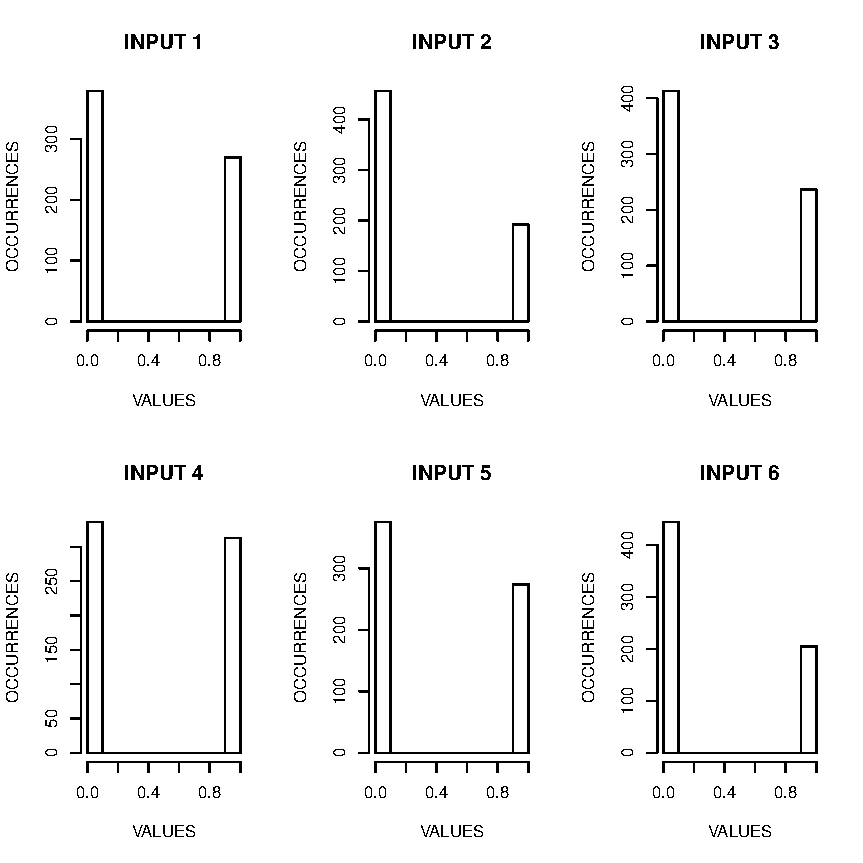
\includegraphics[width=0.7\columnwidth]{image/input1_6.pdf}
  \caption{First six input variables}
  \label{fig:input16}
\end{figure}
%\begin{figure}[h]
%  \vspace{-0.2cm}
%  \centering
%  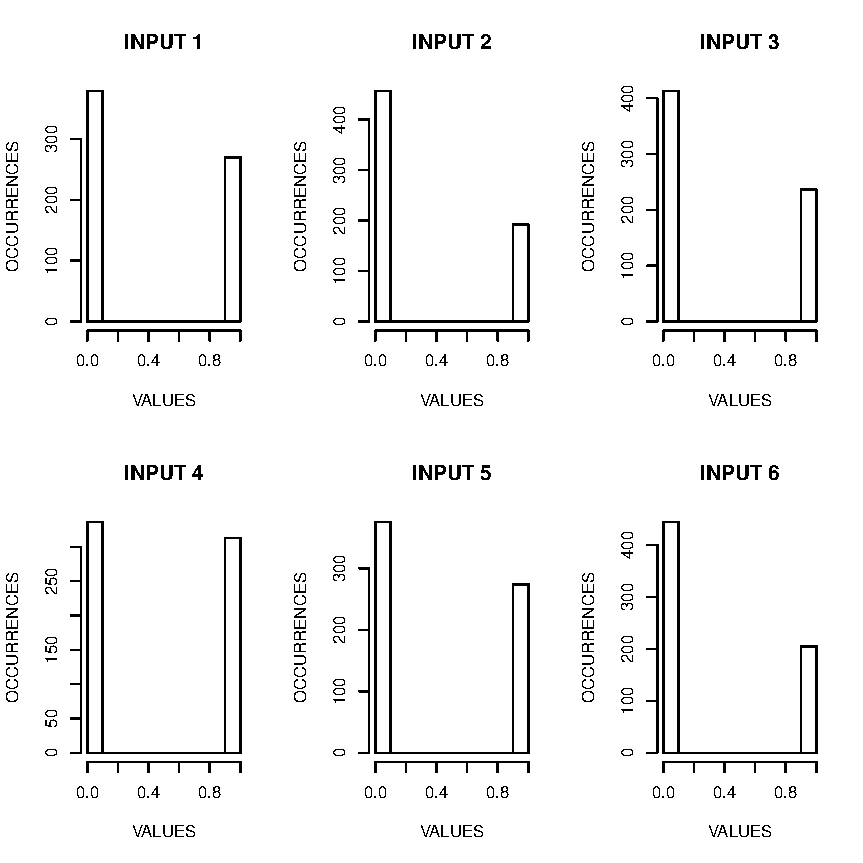
\includegraphics[width=0.7\columnwidth]{image/input1_6.pdf}
%  \caption{Primeiras seis variáveis de entrada}
%  \label{fig:input16}
%\end{figure}

\begin{figure}[h]
  \vspace{-0.2cm}
  \centering
  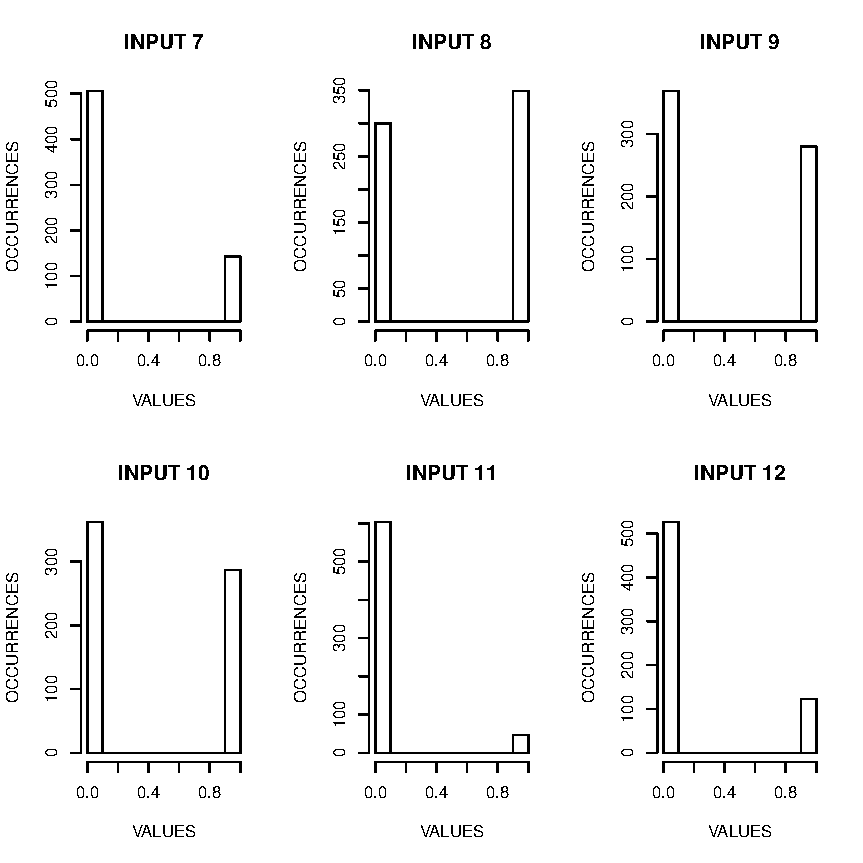
\includegraphics[width=0.7\columnwidth]{image/input7_12.pdf}
  \caption{Last six input variables}
  \label{fig:input712}
\end{figure}
%\begin{figure}[h]
%  \vspace{-0.2cm}
%  \centering
%  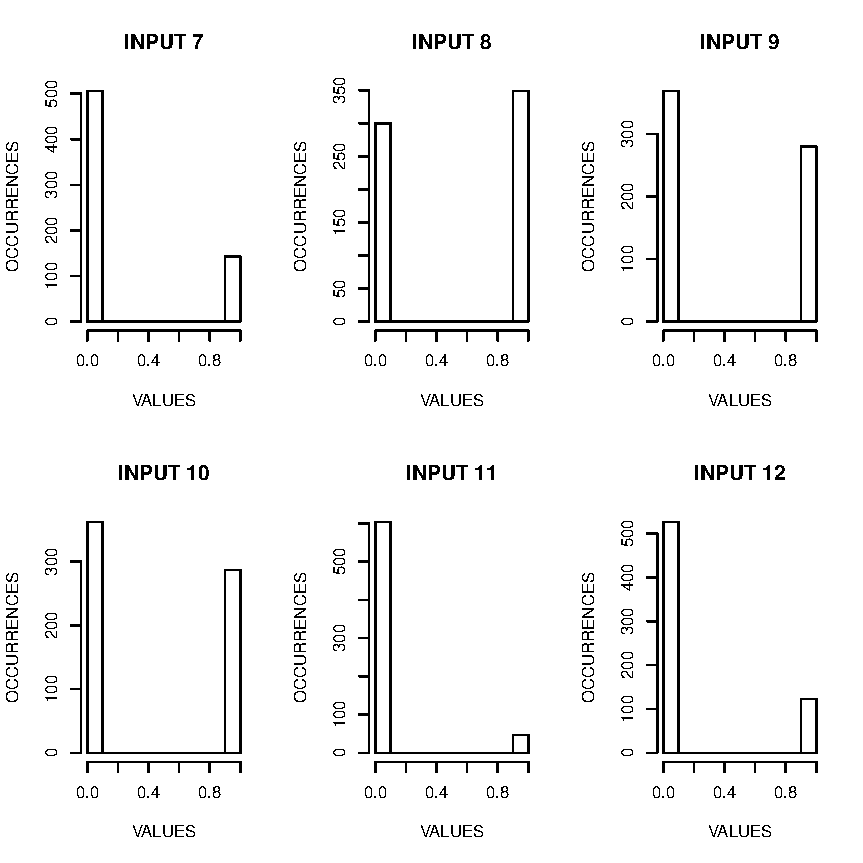
\includegraphics[width=0.7\columnwidth]{image/input7_12.pdf}
%  \caption{Últimas seis variáveis de entrada}
%  \label{fig:input712}
%\end{figure}

\begin{figure}[h]
  \vspace{-0.2cm}
  \centering
  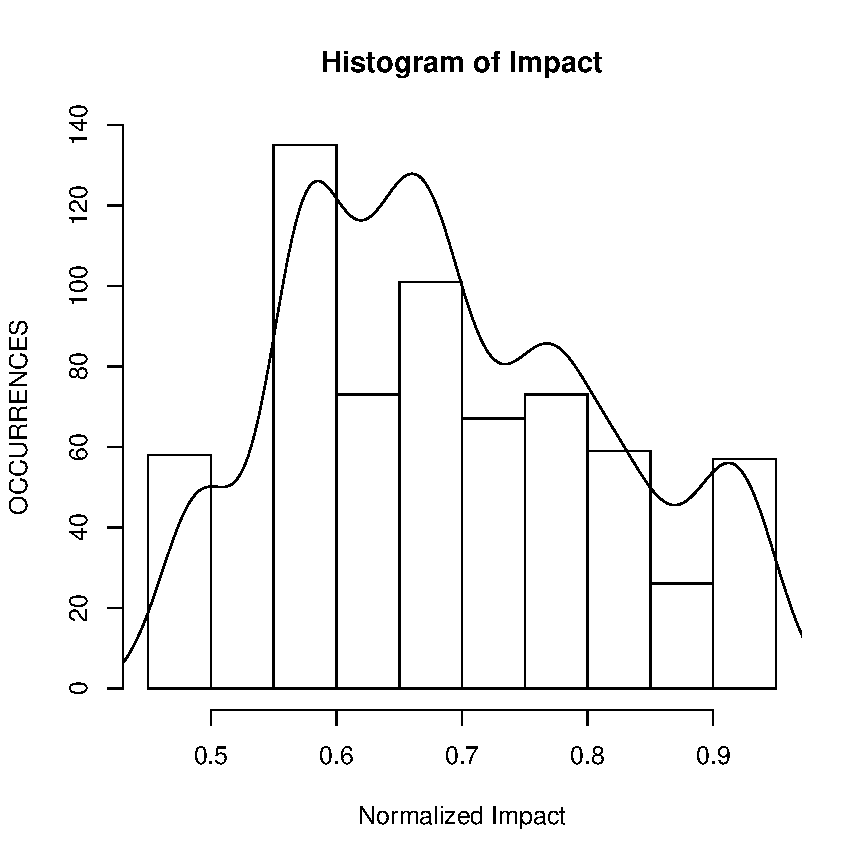
\includegraphics[width=0.5\columnwidth]{image/impact_histogram.pdf}
  \caption{Histogram of impact and shape of the distribution fitting function}
  \label{fig:impacthistogram}
\end{figure}
%\begin{figure}[h]
%  \vspace{-0.2cm}
%  \centering
%  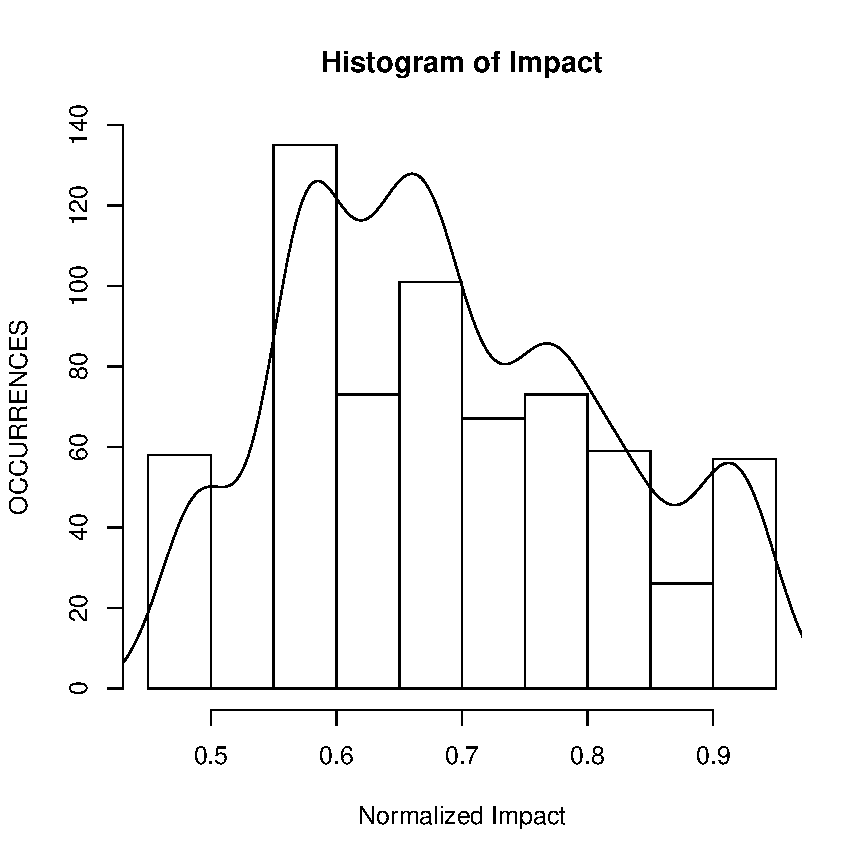
\includegraphics[width=0.5\columnwidth]{image/impact_histogram.pdf}
%  \caption{Histograma do impacto e forma da função de distribuição de ajuste}
%  \label{fig:impacthistogram}
%\end{figure}

For our purpose, PERIL was split into three disjoint subsets - training, cross-validation and test subsets, corresponding to fifty, twenty-five and twenty five percent of the dataset, respectively. \textit{Split-sample} cross-validation method was used for MLRM and RTM models. Whereas \textit{early stopping} and \textit{split-sample} cross-validation methods were combined and used for MLP, SVM, RBF and ANFIS training \cite{priddy2005artificial}.
%Para o nosso objetivo, PERIL foi dividida em três subconjuntos disjuntos - treinamento, validação cruzada e teste, correspondendo a cinquenta, vinte e cinco porcento e o restante da base de dados, respectivamente. O método de validação-cruzada com divisão de amostras foi utilizado tanto para o MRLM e o MRA quanto para o MLP, SVM, RBF e o ANFIS; sendo que para esses o método da parada prematura também foi utilizada no treinamento \cite{priddy2005artificial}.

\section{State of art models}
\label{sec:models}

%Nesta seção, são descritos as configurações adotadas para a experimentação dos modelos de estado da arte.
In this section, adopted configurations for experiments of state of art models are described.

\subsection{Monte Carlo Simulation}

MCS technique used the entire dataset in order to increase the performance prediction. It was filtered only the possible real outcomes to generate the calculated outcome. Towards this decision, we have reduced prediction issues and have improved its performance.
%A Simulação de Monte Carlo utilizou a base de dados inteira com o objetivo de aumentar o desempenho do modelo durante a previsão. Além disso, foram filtradas somente as saídas possíveis para uma dada entrada para que uma nova saída pudesse ser calculada. Através desse método, o desempenho da estimativa do impacto dos riscos foi melhorado.

\subsection{PERT Analysis}

%A Análise PERT também utilizou a base de dados inteira e somente as saídas possíveis para uma determinada entrada foi utilizada no cálculo da nova saída, tal qual a SMC. A partir dessa configuração o resultado desse modelo foi melhorado, em comparação com o cenário em que a base de dados não foi filtrada.
PERT analysis also used the entire database and only possible output for a given input was selected to calculate the new output, like MCS. From this setup the result of this model has been improved compared to a scenario where the database was not filtered.

\section{Linear Regression Model}

%Nesta seção, são descritas as configurações adotadas para a experimentação com os modelos de regressão linear. 
In this section, the configurations adopted for experimentation with linear regression models are described.

The source code of MLR models were adapted from Torgo \cite{torgo2003data} in order to perform linear regression model training, cross-validation, outcome prediction and MAE evaluation. MLR and RTM models were analyzed statistically to define the baseline linear regression model for further analysis.
%O código-fonte dos modelos de regressão linear foram adaptados de Torgo \cite{torgo2003data} para realizar o treinamento, validação cruzada, teste e avaliação da Raiz do Erro Médio Quadrático. Os modelos MRLM e MAR foram comparados estatisticamente para que se pudesse definir um modelo de regressão linear padrão para estudos futuros com a base de dados correspondente.

%Um estudo com esses modelos de regressão linear são necessários porque não há um estudo base para a estimativa de impactos de risco utilizando a PERIL. Portanto, durante os experimentos, a avaliação do melhor modelo de regressão linear tem como objetivo definir um limite superior de valores da REMQ. Isso significa que os modelos que obtiverem erros acima desse limite superior são insatisfatórios.
A study with these linear regression models are necessary because there is not a standard study to estimate risk impacts using PERIL. Therefore, during the experiments, the evaluation of the best linear regression model aims to define an upper limit value of RMSE. That means models who get errors above this upper limit are unsatisfactory.

\subsection{Multiple Linear Regression Model}

%O MRLM é o modelo de regressão linear mais simples possível para a estimativa do impactos dos riscos apresentados na PERIL. Após a otimização do Modelo de Regressão Linear através da seleção das melhores variáveis de entrada utilizando o critério \textit{Akaike Information Criterion}(AIC) sete das onze variáveis foram selecionadas, além do termo independente.
MLRM is a simplest possible model for impact estimation and risks in PERIL linear regression. After optimizing of Linear Regression Model by selecting the best input variables based on Akaike Information Criterion (AIC), seven of eleven variables were selected plus the independent term.

\subsection{Regression Tree Model}

%O modelo MRA constrói uma árvore de classificação das variáveis de entrada, nesse caso pode não ser necessário utilizar todas as variáveis de entrada para a construção do modelo. Ele tenta obter erros de previsão menores que o MRLM através da seleção das variáveis de entrada que têm maior correlação linear com a saída. Na Seção \ref{cap:experiments}, três modelos de árvore de regressão foram analisados com o modelo de regressão linear múltipla.
MRA model builds a classification tree of input variables, in this case it may not be necessary to use all input variables for model construction. It tries to get errors smaller than MLRM through the selection of input variables that have linear correlation with predicted output. In Section \ref{cap:experiments}, three regression tree models were analyzed with a multiple linear regression model.

\section{Particle Swarm Optimization}

%Para o PSO, os parâmetros descritos na Tabela \ref{tab:pso_configuration} foram utilizados. A variação do PSO utilizada é aquela que implementa o coeficiente de constrição de Clerk, como explicado anteriormente.
For PSO, the parameters described in Table \ref{tab:pso_configuration} were adopted. PSO variant utilized is the one that implements constriction Clerk coefficient, as explained previously.

\begin{table}[h]
\caption{PSO Parameters.}\label{tab:pso_configuration} \centering
\begin{tabular}{|c|c|}
  \hline
  Parameter & Value \\
  \hline
  Cognitive Coeficient & 2.05 \\
  \hline
  Social Coeficient & 2.05 \\
  \hline
  Inertia Factor & 0.8 \\
  \hline
  Particles Number & 30 \\
  \hline
  Cycles Number & 600 \\
  \hline
\end{tabular}
\end{table}

%Cada partícula no PSO representa uma configuração candidata. A função de avaliação das partículas é a REMQ de trinta avaliações da rede neural artificial analisada cujos parâmetros são cada partícula. Os parâmetros das redes MLP, SVM e RBF são determinados após a execução desse algoritmo.
Each particle in PSO is a candidate configuration. The fitness function of particles is the RMSE of thirty evaluations of artificial neural network in case whose parameters are each particle. The parameters of the MLP, SVM and RBF networks are determined after the execution of this algorithm.

\section{Artificial Neural Networks}
\label{sec:rnas}

%Nesta seção, descrevemos as configurações das redes neurais artificiais utilizadas nesse estudo.
In this section, it is described the settings of artificial neural networks in this study.

\subsection{MLPs}

%Algumas variações do modelo da MLP foram utilizadas nesse estudo. Diversos parâmetros podem ser alterados como: a quantidade de camadas escondidas, quantidade de neurônios escondidos em cada camada escondida, taxa de aprendizado, momento, número máximo de ciclos de treinamento e regra de aprendizado. Um modelo MLP utilizado nesse estudo é apresentado na Figura \ref{fig:mlp_example}. Nesse modelo tem-se dez neurônios escondidos em uma única camada escondida.
Some variations of the MLP model were used in this study. Several parameters can be modified such as the number of hidden layers, number of hidden neurons in each hidden layer, learning rate, momentum, maximum number of training cycles and learning rule. A MLP model used in this study is shown in Figure \ref{fig:mlp_example}. This model has are ten hidden neurons in a single hidden layer.

\begin{figure}[!h]
  \vspace{-0.2cm}
  \centering
  \def \svgwidth{0.55\columnwidth}
  \input{image/mlp.pdf_tex}
  %\caption{Um modelo MLP utilizado no estudo.}
  \caption{A MLP model utilized in this study.}
  \label{fig:mlp_example}
\end{figure} 

%A quantidade de camadas escondidas estudadas foram uma e duas camadas. O número de neurônios na(s) camada(s) escondida(s), a taxa de aprendizado e o momento foram determinados por um algoritmo de otimização como o PSO para aumentar a precisão na estimativa de erros. Para as análises, o número máximo de ciclos de treinamento foi configurado para seiscentos.
Hidden layers were single and double layer. The number of neurons in hidden(s) layer(s), the learning rate and momentum have been determined by an optimization algorithm such as PSO to increase the accuracy of errors estimation. For analyzes, the maximum number of training cycles was set to six hundred.

Learning rate, momentum and neurons in hidden layer varied from values presented in Table \ref{tab:mlp_configuration_investigation}. A better parameters configuration solution is shown in Table \ref{tab:mlp_best_configuration}. Figure \ref{fig:mlpmodelstudy} presents MLP model with the better configuration for PERIL. The model contains ten neurons in hidden layer.
%A taxa de aprendizado, momento e a quantidade de neurônios escondidos variam de acordo com os valores apresentados na Tabela \ref{tab:mlp_configuration_investigation}.

\begin{table}[h]
\caption{Parameters intervals to MLP model.}\label{tab:mlp_configuration_investigation} \centering
\begin{tabular}{|c|c|c|}
  \hline
  Parameter & Min. Value & Max. Value \\
  \hline
  Momentum & 0.1 & 0.9 \\
  \hline
  Learning rate & 0.1 & 0.9 \\
  \hline
  Hidden Neurons & 1 & 100 \\
  \hline
\end{tabular}
\end{table}
%\begin{table}[h]
%\caption{Intervalos de parâmetros para a MLP.}\label{tab:mlp_configuration_investigation} \centering
%\begin{tabular}{|c|c|c|}
 % \hline
 % Parâmetros & Valor Mínimo & Valor Máximo \\
  %\hline
  %Momento & 0.1 & 0.9 \\
  %\hline
  %Taxa de Aprendizado & 0.1 & 0.9 \\
  %\hline
  %Neurônios Escondidos & 1 & 100 \\
  %\hline
%\end{tabular}
%\end{table}

%Por fim, as regras de aprendizado utilizadas nesse estudo são \textit{Backpropagation}, Levenberg-Marquardt, BFGS Quasi-Newton, \textit{Resilient Backpropagation}, \textit{Polak-Ribiére Conjugate Gradient}, Gradiente Conjugado Escalonado e \textit{One Step Secant}.
Finally, the learning rules used in this study are Backpropagation, Levenberg-Marquardt, BFGS Quasi-Newton, Resilient Backpropagation, Polak-Ribiére Conjugate Gradient, Scaled Conjugate Gradient e One Step Secant.

%Em particular, uma MLP, chamada "MLPRegressor", que tem uma camada escondida e cuja regra de aprendizado tem o objetivo de minimizar o erro médio quadrático mais uma penalidade quadrática através do método BFGS Quasi-Newton teve um melhor desempenho que as demais variações.
In particular, a MLP called "MLPRegressor" which has one hidden layer and whose learning rule aims to minimize the mean square error over a quadratic penalty through the BFGS Quasi-Newton method performed better than others variations.

\subsection{SVM}

%O algoritmo SVM para regressão utilizado é o SMOReg. Nesse algoritmo RegSMOImproved é o algoritmo de otimização e PolyKernel é a função de kernel como descrito em \cite{Shevade1999}. O pseudo-código para esse algoritmo é apresentado no Algoritmo \ref{code:svm}.
SVM algorithm for regression used is SMOReg. In this algorithm RegSMOImproved is the optimization algorithm and PolyKernel is the kernel function as described in \cite{Shevade1999}. The pseudo-code for this algorithm is presented in Algorithm \ref{code:svm}.

\begin{algorithm}[H]
%\SetAlgoLined
\label{alg:pseudocodigoPSO}
\Inicio{
    inicializar as partículas no espaço de busca dispostas aleatoriamente\;
    \ParaCada{partícula}{
        extrair o \textit{fitness} inicial\;
        estabelecer seu $\vec{P}_{best}$ inicial\;
    }
    estabelecer o $\vec{G}_{best}$ inicial\;
    \Enqto{critério de parada não é atingido}{
        \ParaCada{partícula}{
            atualizar a velocidade da partícula\;
            atualizar a posição da partícula\;        
            extrair o \textit{fitness}\;
            atualizar seu $\vec{P}_{best}$\;        
        }
        atualizar o $\vec{G}_{best}$\;
    }
    \Retorna{$\vec{G}_{best}$}
}
\caption{Pseudocódigo do PSO}
\end{algorithm}

\begin{small}
\label{code:svm}
\begin{verbatim}
 Begin
     peril <- read_file();
     peril_train <- partition(peril, 0, 50);
     peril_crossvalidation <- partition(peril, 50, 75);
     peril_test <- partition(peril, 75, 100);
     smo <- SMOReg();
     options <- [peril_train, peril_crossvalidation, 
                 RegSMOImproved, PolyKernel]
     SMOReg.runClassifier(smo, options);
     for instance in peril_test:
          calculated <- smo.classifyInstance(instance);
          wished <- instance.classValue();
          REMQ <- REMQ + (wished - calculated)^2
     end
     n <- peril_test.size();
     REMQ <- REMQ/n;
     REMQ <- sqrt(REMQ);
 End
\end{verbatim}
\end{small}

%No Algoritmo \ref{code:svm}, os dados são lidos a partir de um arquivo, dividido nos subconjuntos treinamento, validação cruzada e teste. Instanciar o modelo de regressão SMOReg, executar o treinamento do modelo, gerar a saída calculada e calcula o REMQ a partir da saída real e calculada. Esse algoritmo é utilizado como a função de otimização para o algoritmo de otimização por enxames.
In Algorithm \ref{code:svm}, data is read from a file, divided into training, cross validation and testing subsets. SMOReg regression model is instantiated, training is performed, calculated outcome is generated and the RMSE from the real and estimated output is calculated. This algorithm is used in fitness function for swarm optimization algorithm.

\subsection{RBF}

%A rede neural RBF utilizada é a RBFRegressor, ela minimiza o erro quadrático através do método BFGS. Os centros iniciais das gaussianas são encontrados utilizando SimpleKMeans, um algoritmo que implementa K-Médias. O sigma inicial é configurado para a maior distância entre qualquer centro e o vizinho mais próximo no conjunto de centros. O parâmetro de cume é usado para penalizar o tamanho dos pesos na camada de saída, o qual implementa uma combinação linear simples. O número de funções de base pode também ser especificado. Para esse estudo somente um sigma global é utilizado para todas as funções de base. O pseudo-código para esse algoritmo é apresentado no Algoritmo \ref{code:rbf}.
RBF neural network used is RBFRegressor, it minimizes the square error by BFGS method. The initial Gaussian centers are found using SimpleKMeans, which implements a K-Means algorithm. The initial sigma is set to the longest distance between any center and the nearest neighbor in the set of centers. The ridge parameter is used to penalize the size of the weights in the output layer, which implements a simple linear combination. The number of basis functions can also be specified. For this study only a global sigma is used for all basis functions. The pseudo-code for this algorithm is presented in Algorithm \ref{code:rbf}.

\begin{small}
\label{code:rbf}
\begin{verbatim}
 Begin
     peril <- read_file();
     peril_train <- partition(peril, 0, 50);
     peril_crossvalidation <- partition(peril, 50, 75);
     peril_test <- partition(peril, 75, 100);
     rbf <- RBFRegressor();
     options <- [peril_train, peril_crossvalidation, peril_test]
     RBFRegressor.runClassifier(rbf, options);
     for instance in peril_test:
          calculated <- rbf.classifyInstance(instance);
          wished <- instance.classValue();
          REMQ <- REMQ + (wished - calculated)^2
     end
     n <- peril_test.size();
     REMQ <- REMQ/n;
     REMQ <- sqrt(REMQ);
 End
\end{verbatim}
\end{small}

In Algorithm \ref{code:rbf}, data is read from a file, divided into training, cross validation and testing subsets. The instantiated regression model is  SMOReg, training is overcame, calculated output is generated and RMSE is obtained from the real and estimated output. This algorithm is used in fitness function for swarm optimization algorithm.
%No Algoritmo \ref{code:rbf}, os dados são lidos a partir de um arquivo, dividido nos subconjuntos treinamento, validação cruzada e teste. O modelo de regressão SMOReg é instanciado, o treinamento do modelo é executado, a saída calculada é gerada e a REMQ é obtida a partir da saída real e calculada. Esse algoritmo é utilizado como a função de otimização para o algoritmo de otimização por enxames.

\subsection{ANFIS}

%O ANFIS é um sistema neuro-fuzzy implementado no Matlab por Sugeno \cite{jang1997neuro}. ANFIS usa um algoritmo de aprendizado híbrido para identificar parâmetros do sistema de inferência fuzzy Sugeno. Ele aplica uma combinação do método dos mínimos quadrados e o método do gradiente descendente \textit{backpropagation} para o treinamento dos parâmetros da função de pertinência do sistema de inferência fuzzy. O sistema de inferência fuzzy utilizado foi o genfis2, já que há um número grande de variáveis de entrada. O pseudo-código para esse algoritmo é apresentado no Algoritmo \ref{code:anfis}.
ANFIS is a neuro-fuzzy system implemented in Matlab by Sugeno \cite{jang1997neuro}. ANFIS uses a hybrid learning algorithm to identify parameters of Sugeno fuzzy inference system. It applies a combination of the method of least squares and gradient descent backpropagation for training the parameters of the membership function of the fuzzy inference system method. The fuzzy inference system used is genfis2, since there is a large number of input variables. The pseudo-code for this algorithm is presented in Algorithm \ref{code:anfis}.

\begin{small}
\label{code:anfis}
\begin{verbatim}
 Begin]
     inputs = csvread(peril,0,0,[0,0,648,10])
     targets = csvread(peril,0,11)
     tData = [inputs targets];
     in_fis = genfis2(inputs,targets, 0.7);
     trainOpts = [100,0.1,0.01,0.9,1.1]
     displayOpts = [1,1,1,1];
     chkData = []
     [fis,error,stepsize,chkFis,chkErr] = 
          anfis(tData,in_fis,trainOpts,displayOpts,
          chkData,1);
     for err in error:
          REMQ <- REMQ + (err)^2
     end
     n <- peril.size();
     REMQ <- REMQ/n;
     REMQ <- sqrt(REMQ);
 End
\end{verbatim}
\end{small}

In Algorithm \ref{code:svm}, data were read from file. The fuzzy inference system is instantiated, training is performed, error is generated and RMSE is obtained from the real and estimated outcome. This algorithm is used as fitness function for swarm optimization algorithm.
%No Algoritmo \ref{code:anfis}, os dados de entrada e saída são lidos a partir de um arquivo. O sistema de inferência fuzzy é instanciado, o treinamento do modelo é executado, o erro é gerado e a REMQ é obtida a partir da saída real e calculada. Esse algoritmo é utilizado como a função de otimização para o algoritmo de otimização por enxames.

\pagebreak